The guiding trajectory is modeled as the connected lines between $n$ waypoints $g_1,...,g_n$. To calculate the progress at position $p$ we define the closest point on the trajectory as $\psi(p)$ and its corresponding line segment index as $l(p)$ as 
\begin{align}
\label{equ:progress_computation}
    l(p),\psi(p) &= \text{arg min}_{l(p),\psi(p)} \|p - \psi(p)\| \\
    \text{s.t. } & \psi(p) = g_{l(p)} + t (g_{l(p)+1} -  g_{l(p)}), \nonumber \\
     &t = \frac{(p - g_{l(p)}) \cdot (g_{l(p)+1} -  g_{l(p)})}{\|g_{l(p)+1} -  g_{l(p)}\|^2} , \nonumber \\
     &l(p) \in \{1,..,n-1\}, t \in [0,1]. \nonumber
\end{align}
The computation of the progress in time step $t$ is illustrated in Figure \ref{fig:trajectory}. 

\begin{figure}[b]
    \centering
    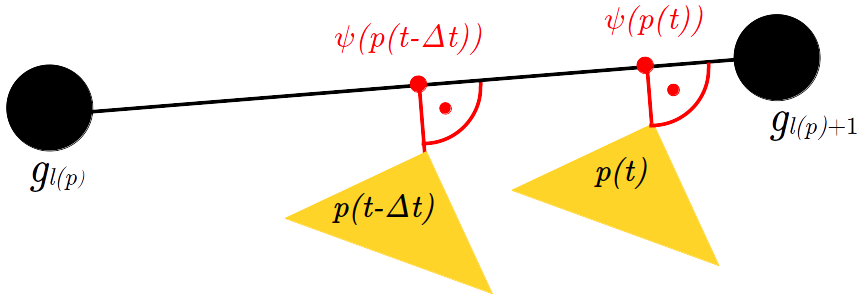
\includegraphics[width=0.3\textwidth]{images/trajectory.png}
    \caption{Illustration of trajectory with two waypoints. The nearest point $\psi(p)$ on trajectory from drone at position $p$ and its corresponding line segment index $l(p)$ is used to calculate the progress in each time step $\Delta t$ and the reached distance.}
    \label{fig:trajectory}
\end{figure}

The reward function consists of five main parts: encouraging progression along the trajectory in every time step, rewarding the overall reached distance along the trajectory, rewarding reached waypoints, penalizing high body rates $\omega$ and penalizing inactivity. This approach is leaned on the work of Penicka et al. \cite{Penicka_2022}.
The total reward function $r(t)$ at time $t$ is defined as 
\begin{align}
\label{equ:reward}
r(t) = k_p r_p(t) + k_s s(p(t)) + k_{wp} r_{wp} + k_\omega \|\omega\| - fall,
\end{align}
with the reached distance along the trajectory $s(p(t))$ and the progress reward at each time step $r_p(t)$ being defined as
\begin{align}
    &s(p) = \sum_{i=1}^{l(p) - 1} \| g_{i+1} - g_i \| + \|\psi(p) - g_{l(p)}\|, \\
    &r_p(t) = s(p(t))-s(p(t- \Delta t)).
\end{align}
The reached distance $s(p(t))$ is part of the reward function to counteract possible singularities due to sharp corners of the trajectory and the minimum distance projection. The reward $r_{wp}$ was payed, if the drone reached a waypoint within a distance $d_{wp}$ smaller than a tolerance $r_{tol}$ for the first time. The term $k_\omega \|\omega\|$ discourages high body rates. The penalty term $fall$ was only subtracted if the drone fell under $0$m due to inactivity. The contribution of each reward part is scaled by the hyperparameters $k_p$, $k_s$, $k_{wp}$ and $k_{\omega}$.